\chapter{Further data analysis}


%TODO include maps of zones, and tables of population and empoyment values etc
%TODO sections and horizonal lines in appendicies
\begin{figure}[H]
\centering
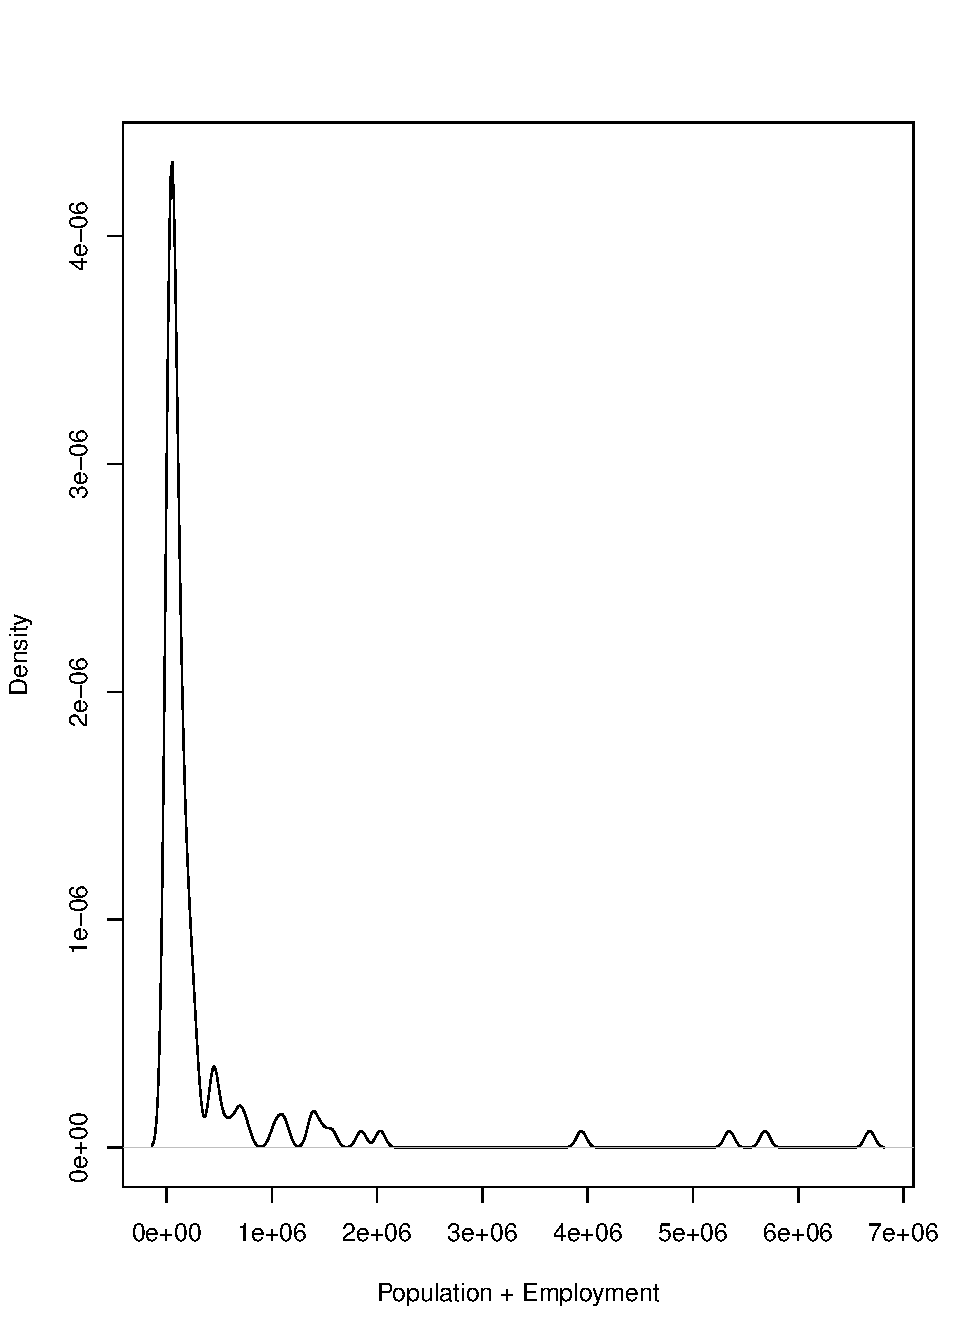
\includegraphics[height=0.6\textheight]{popEmpDensity}
\caption{Long tail and right skew of (population + employment) for each destination}
\label{fig:pop-emp-density}
\end{figure}


\begin{figure}[H]
\centering
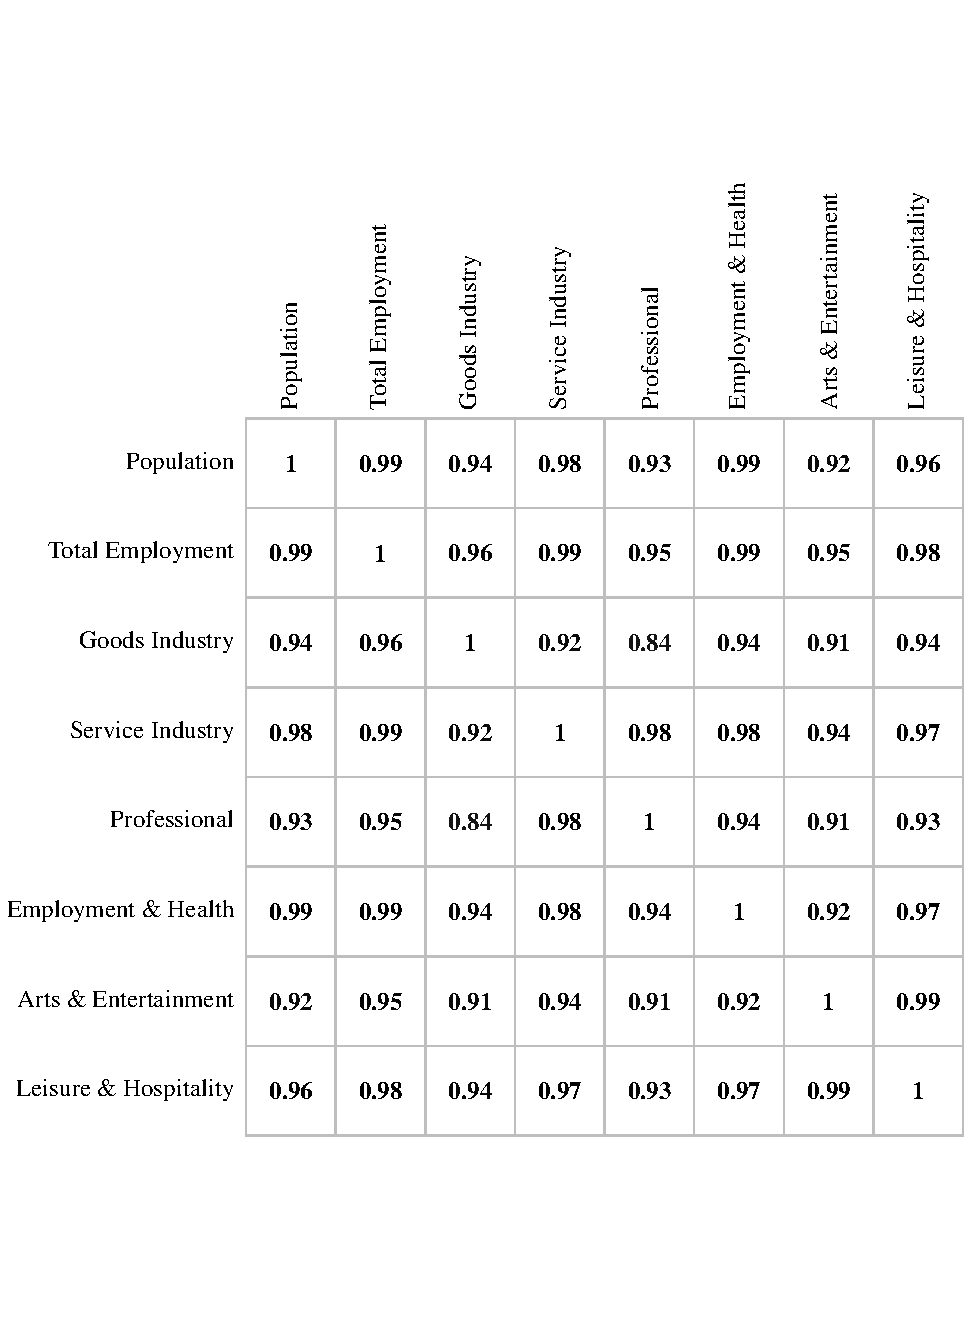
\includegraphics[width=\textwidth]{employment_correlation_plot}
\caption{High correlation between population, employment, and various employment categories across destinations}
\label{fig:pop-emp-correlation}
\end{figure}


\clearpage
\begin{sidewaysfigure}
\centering
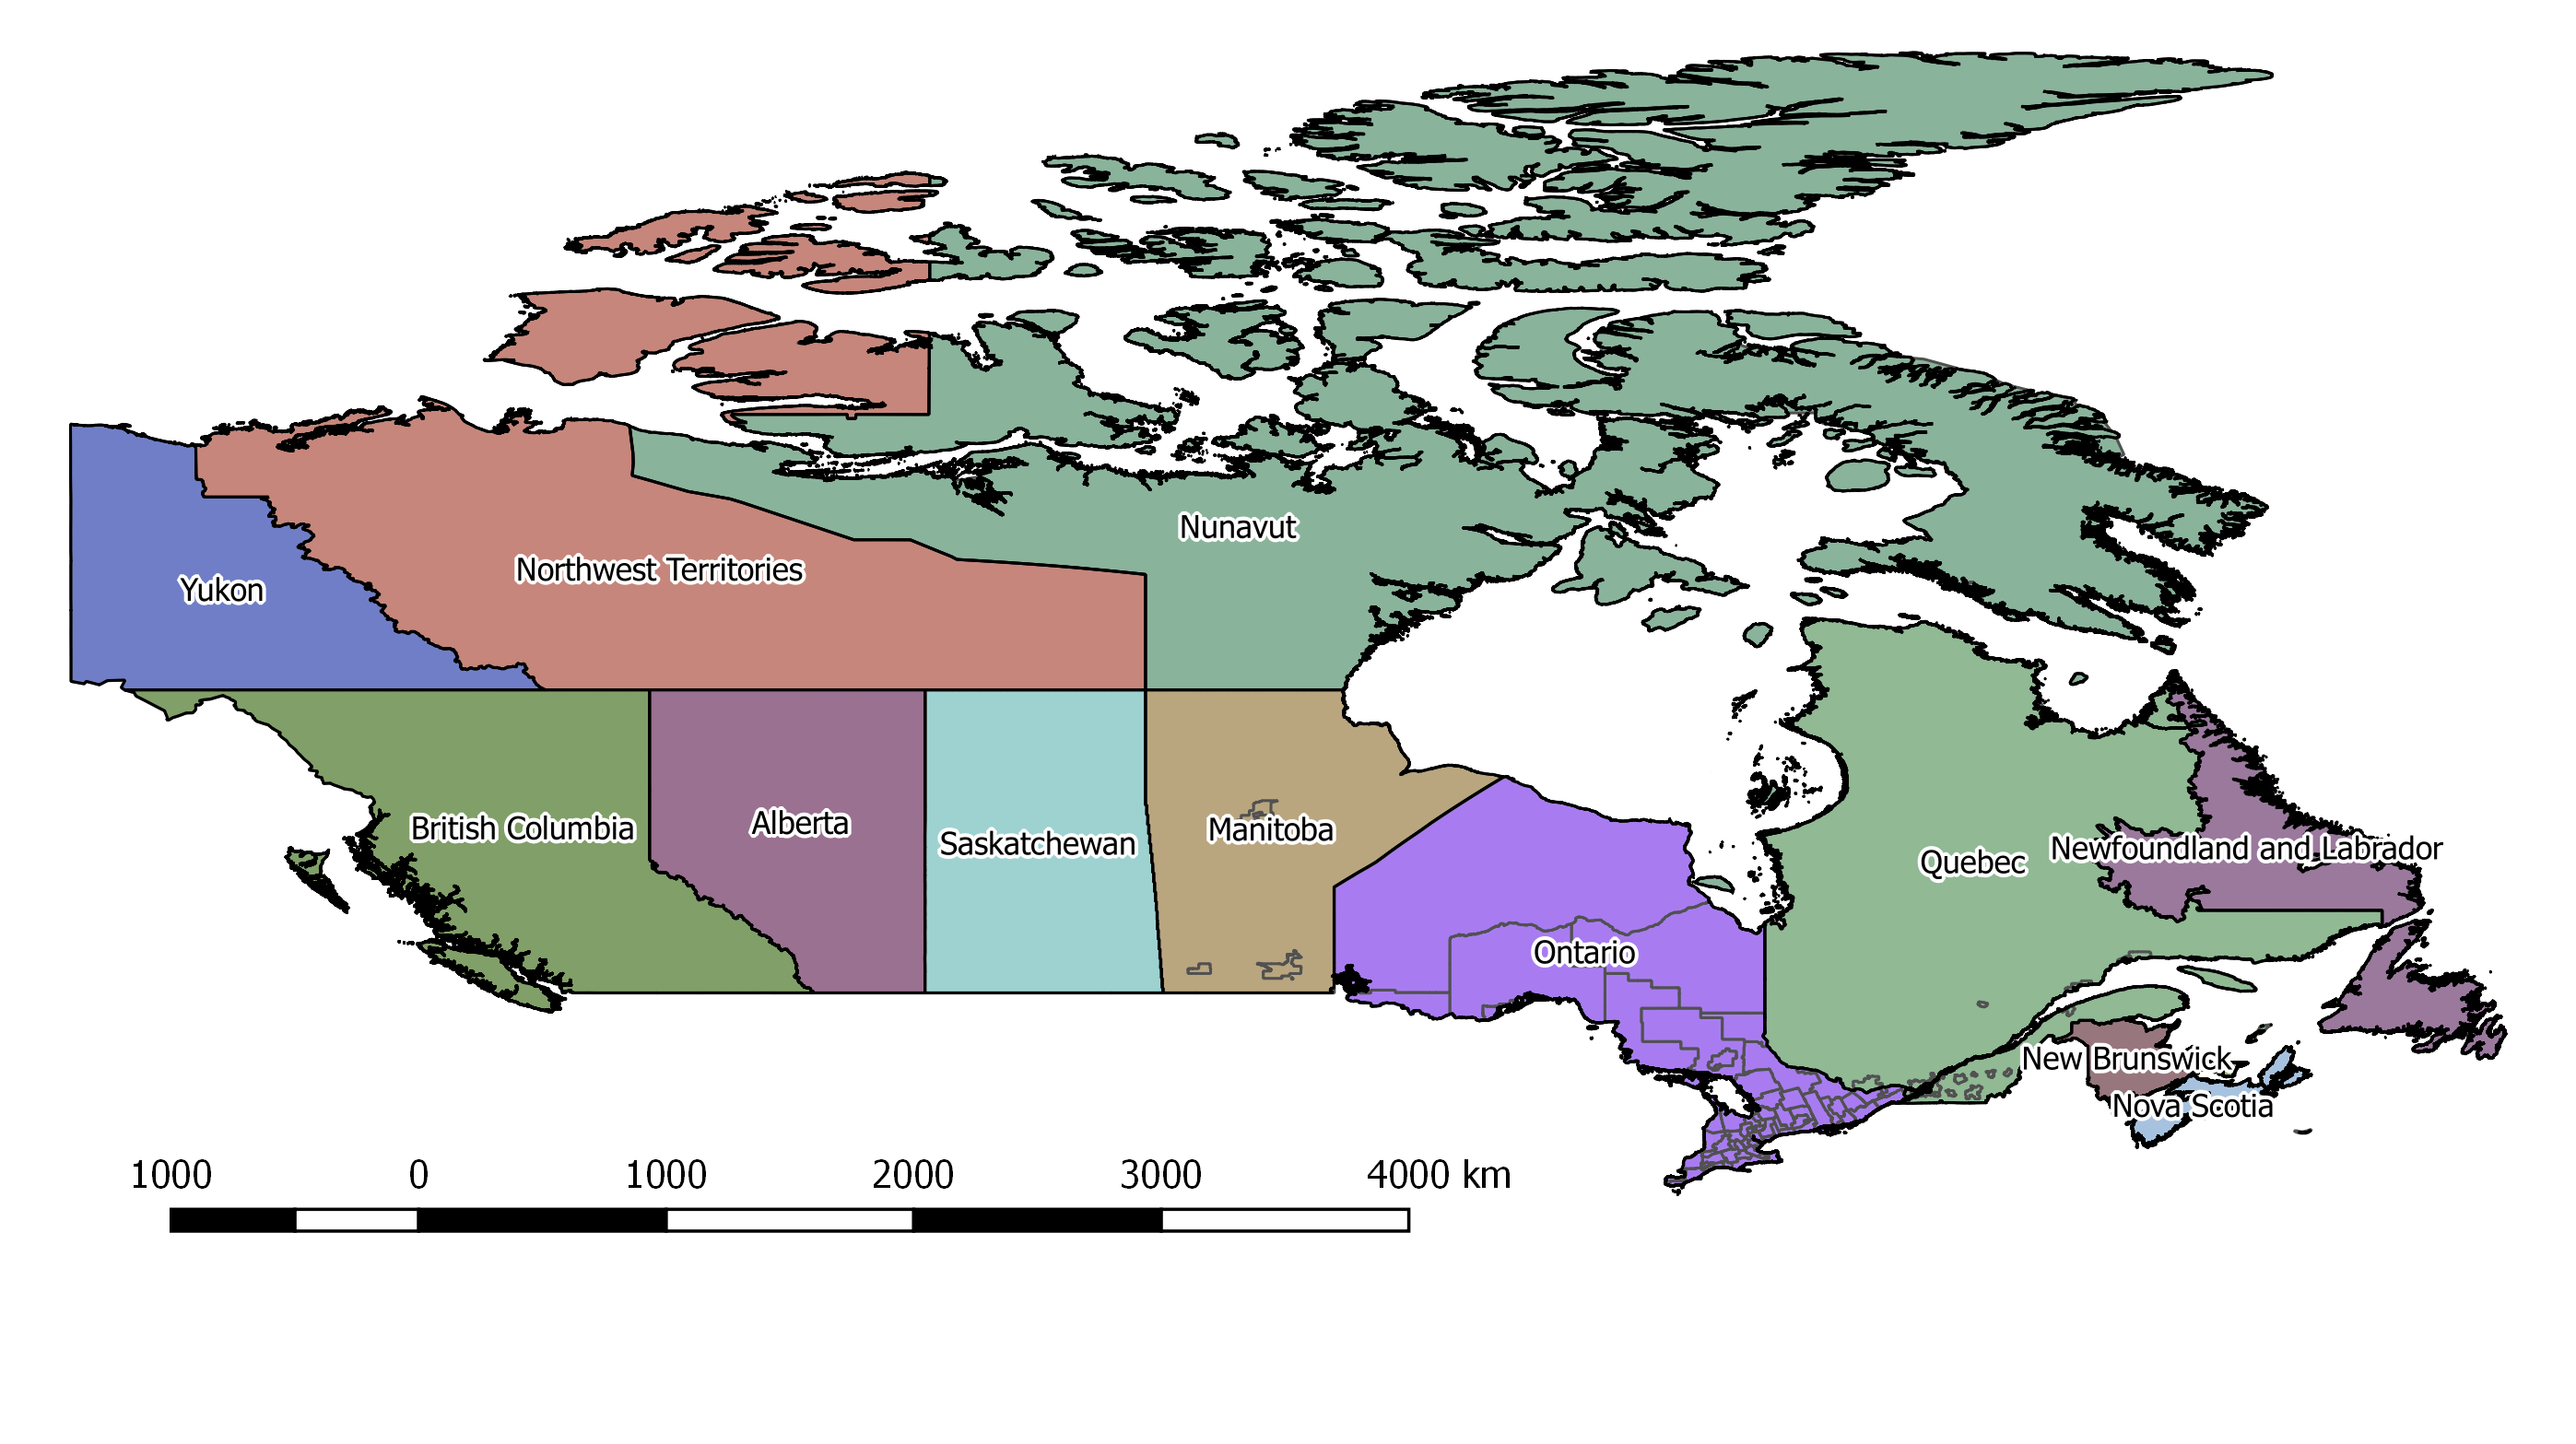
\includegraphics{zones/all_zones}
\caption{Zones by province for Canada}
\label{fig:all-zones}
\end{sidewaysfigure}
\clearpage

\clearpage
\begin{sidewaysfigure}
\centering
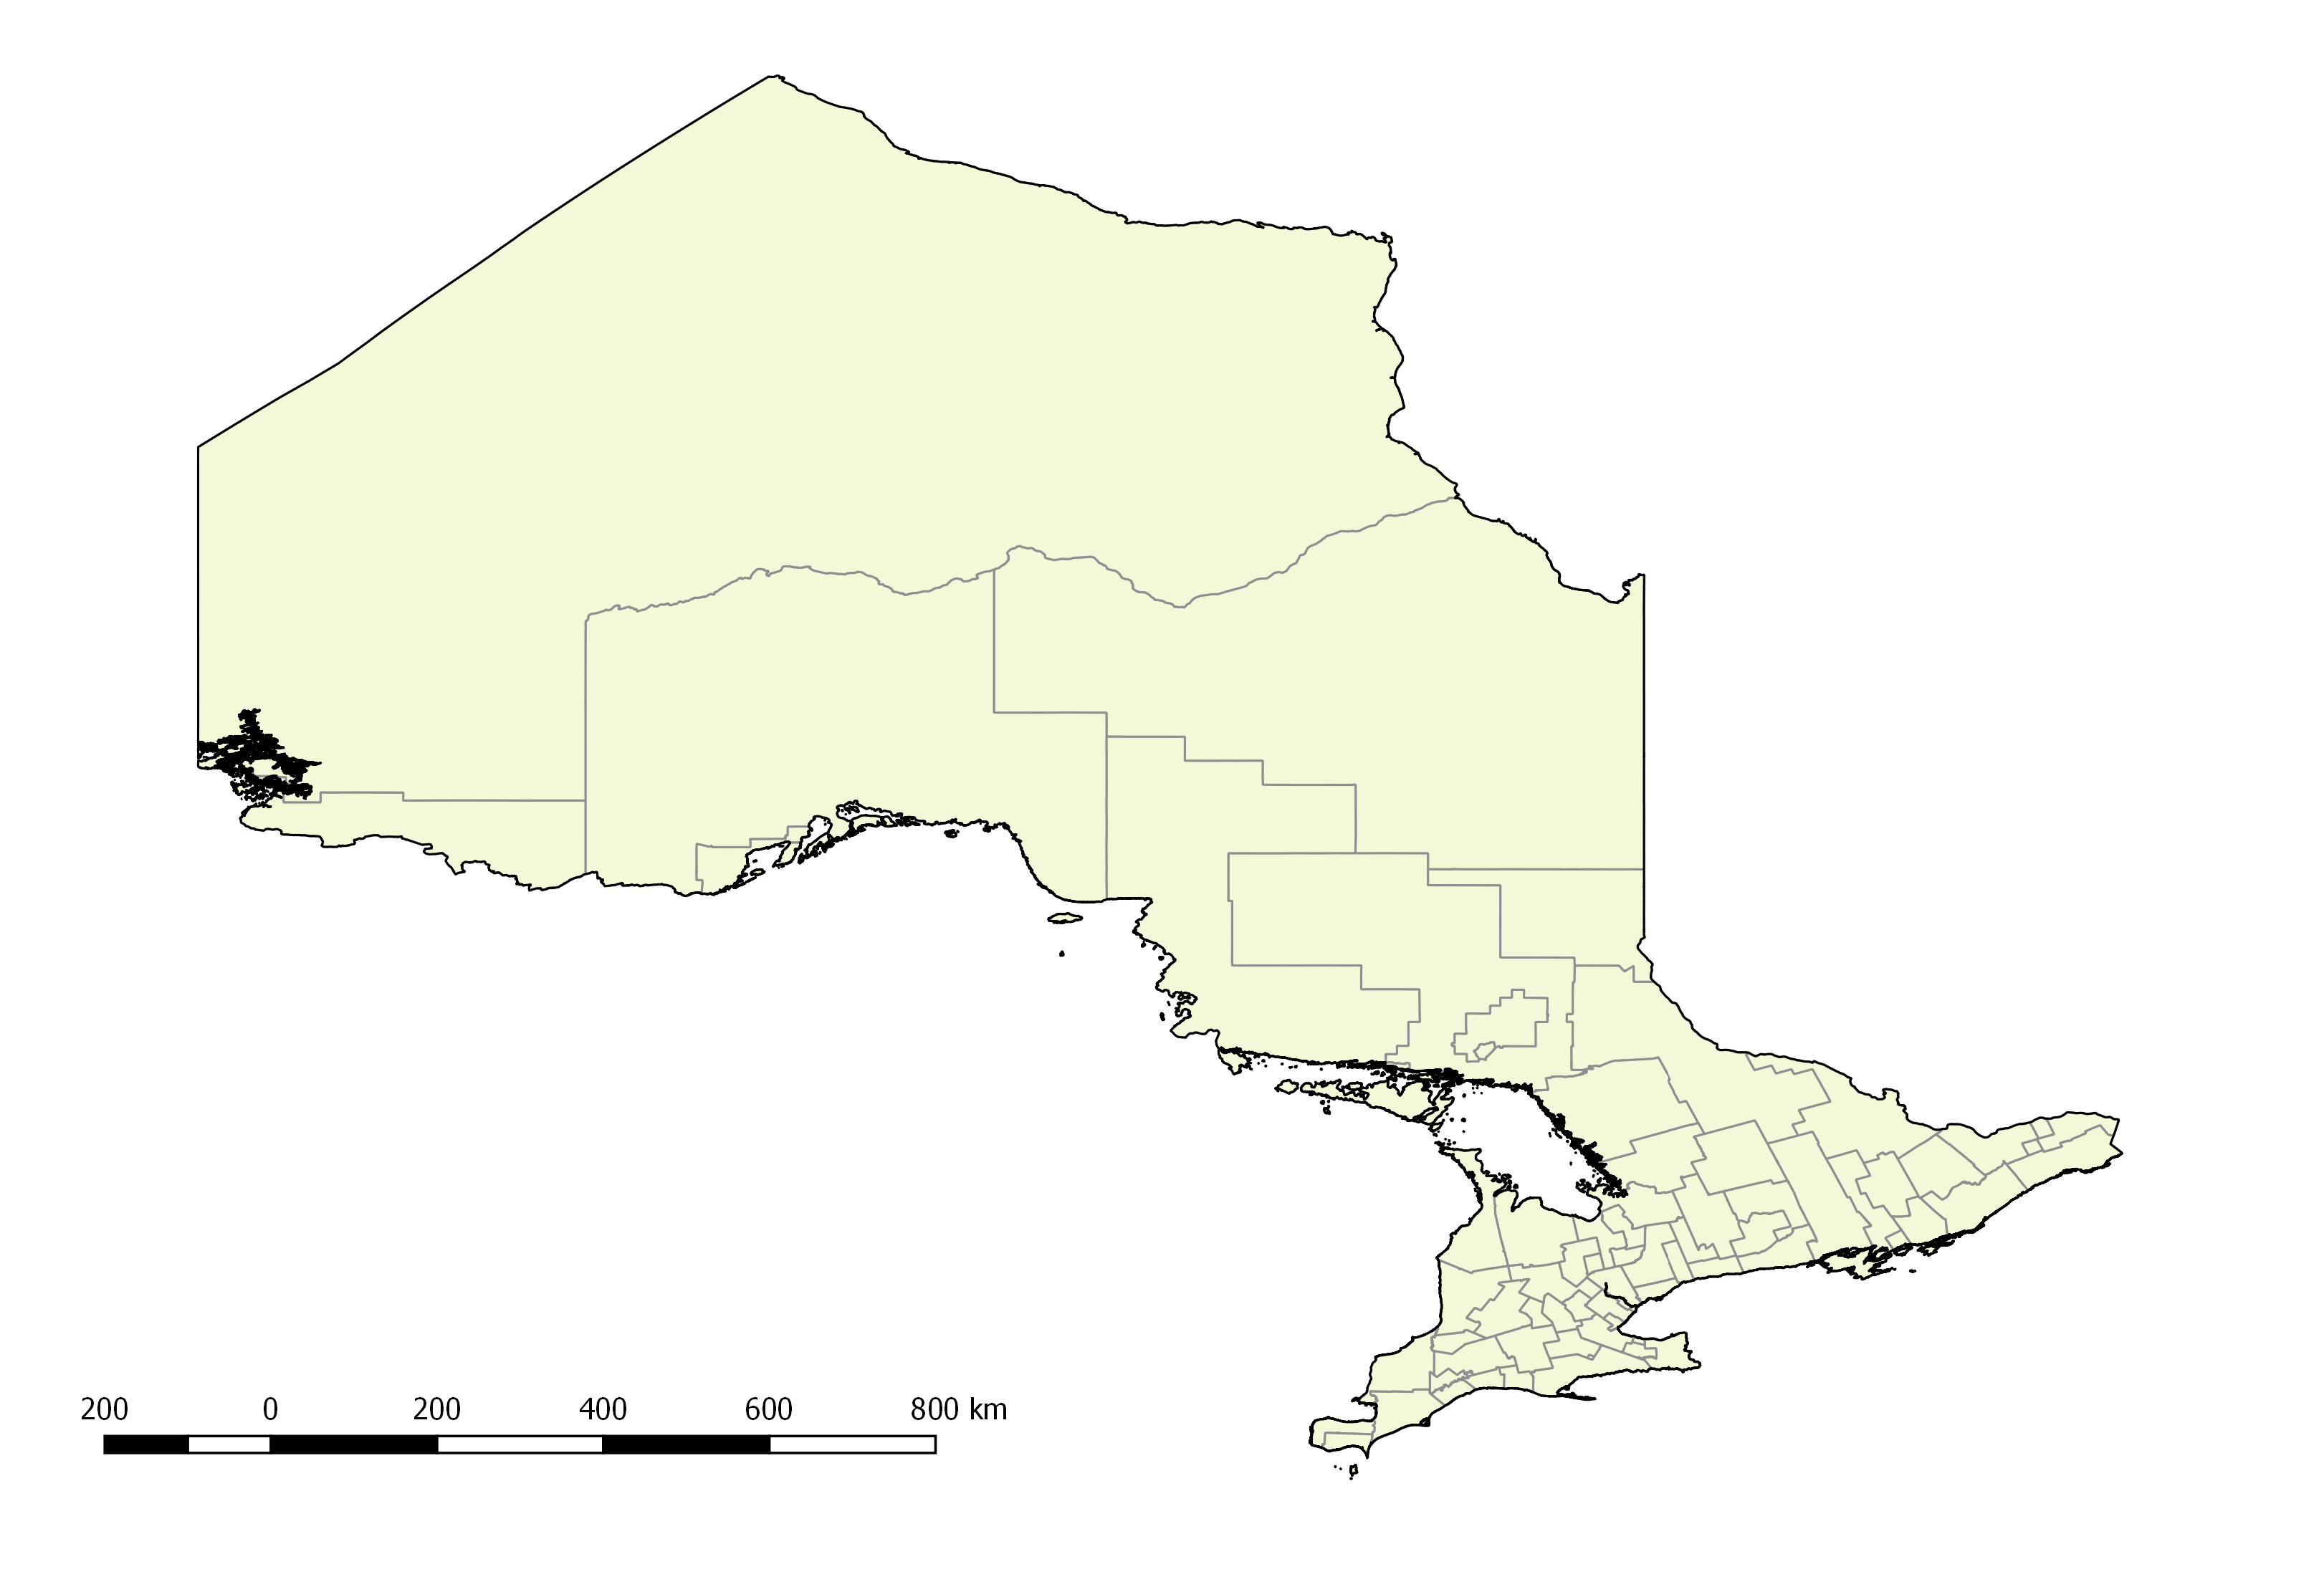
\includegraphics[scale=0.9]{zones/ontario}
\caption{Ontario internal zones}
\label{fig:ontario-zones}
\end{sidewaysfigure}
\clearpage

\chapter{Final model estimation summaries}
\section{Business model strata}
\begin{verbatim}
Call:
mnlogit(formula = f, data = model.inputs[[class]], choiceVar = "alt", 
    weights = trips[[class]]$daily.weight, ncores = 8)

Frequencies of alternatives in input data:
...

Number of observations in data = 6228
Number of alternatives = 84
Intercept turned: OFF
Number of parameters in model = 7
  # individual specific variables = 0
  # choice specific coeff variables = 0
  # individual independent variables = 7

-------------------------------------------------------------
Maximum likelihood estimation using the Newton-Raphson method
-------------------------------------------------------------
  Number of iterations: 6
  Number of linesearch iterations: 7
At termination: 
  Gradient norm = 1.65e-06
  Diff between last 2 loglik values = 0
  Stopping reason: Succesive loglik difference < ftol (1e-06).
Total estimation time (sec): 0.762
Time for Hessian calculations (sec): 0.108 using 8 processors.

Coefficients : 
                     Estimate Std.Error t-value  Pr(>|t|)    
dist_exp             7.794471  0.186216 41.8570 < 2.2e-16 ***
dist_log             0.661833  0.031626 20.9269 < 2.2e-16 ***
civic                0.444640  0.020771 21.4064 < 2.2e-16 ***
mm_inter_no_visit    0.619549  0.041236 15.0244 < 2.2e-16 ***
r_intra              2.003272  0.084420 23.7297 < 2.2e-16 ***
log_hotel            0.151913  0.013159 11.5440 < 2.2e-16 ***
log_sightseeing      0.076344  0.013138  5.8108 6.217e-09 ***
mm_intra_no_business       NA        NA      NA        NA    
visit_log_medical          NA        NA      NA        NA    
niagara                    NA        NA      NA        NA    
summer_log_outdoors        NA        NA      NA        NA    
winter_log_skiing          NA        NA      NA        NA    
---
Signif. codes:  0 ‘***’ 0.001 ‘**’ 0.01 ‘*’ 0.05 ‘.’ 0.1 ‘ ’ 1

Log-Likelihood: -20084, df = 7
AIC:  40182 

\end{verbatim}
\section{Leisure model strata}
\begin{verbatim}

Call:
mnlogit(formula = f, data = model.inputs[[class]], choiceVar = "alt", 
    weights = trips[[class]]$daily.weight, ncores = 8)

Frequencies of alternatives in input data:
...

Number of observations in data = 22909
Number of alternatives = 86
Intercept turned: OFF
Number of parameters in model = 11
  # individual specific variables = 0
  # choice specific coeff variables = 0
  # individual independent variables = 11

-------------------------------------------------------------
Maximum likelihood estimation using the Newton-Raphson method
-------------------------------------------------------------
  Number of iterations: 7
  Number of linesearch iterations: 11
At termination: 
  Gradient norm = 1.656e-05
  Diff between last 2 loglik values = 0
  Stopping reason: Succesive loglik difference < ftol (1e-06).
Total estimation time (sec): 5.856
Time for Hessian calculations (sec): 1.357 using 8 processors.

Coefficients : 
                       Estimate  Std.Error  t-value  Pr(>|t|)    
dist_exp              7.3263663  0.1004878  72.9080 < 2.2e-16 ***
dist_log              0.4784102  0.0222526  21.4991 < 2.2e-16 ***
civic                -0.1741501  0.0111768 -15.5814 < 2.2e-16 ***
mm_inter_no_visit    -0.7638604  0.0213704 -35.7439 < 2.2e-16 ***
mm_intra_no_business -2.4007117  0.0524988 -45.7289 < 2.2e-16 ***
r_intra               0.6512536  0.0426148  15.2823 < 2.2e-16 ***
log_hotel             0.2657799  0.0068486  38.8081 < 2.2e-16 ***
log_sightseeing       0.1430539  0.0066258  21.5906 < 2.2e-16 ***
niagara               0.1245882  0.0028645  43.4932 < 2.2e-16 ***
summer_log_outdoors   0.0390384  0.0056098   6.9589 3.429e-12 ***
winter_log_skiing     0.0997631  0.0042804  23.3069 < 2.2e-16 ***
visit_log_medical            NA         NA       NA        NA    
---
Signif. codes:  0 ‘***’ 0.001 ‘**’ 0.01 ‘*’ 0.05 ‘.’ 0.1 ‘ ’ 1

Log-Likelihood: -77812, df = 11
AIC:  155650 


\end{verbatim}
\section{Visit model strata}
\begin{verbatim}

Call:
mnlogit(formula = f, data = model.inputs[[class]], choiceVar = "alt", 
    weights = trips[[class]]$daily.weight, ncores = 8)

Frequencies of alternatives in input data:
...

Number of observations in data = 33414
Number of alternatives = 86
Intercept turned: OFF
Number of parameters in model = 8
  # individual specific variables = 0
  # choice specific coeff variables = 0
  # individual independent variables = 8

-------------------------------------------------------------
Maximum likelihood estimation using the Newton-Raphson method
-------------------------------------------------------------
  Number of iterations: 8
  Number of linesearch iterations: 30
At termination: 
  Gradient norm = 4.156e-05
  Diff between last 2 loglik values = 0
  Stopping reason: Succesive loglik difference < ftol (1e-06).
Total estimation time (sec): 14.288
Time for Hessian calculations (sec): 1.401 using 8 processors.

Coefficients : 
                       Estimate  Std.Error  t-value  Pr(>|t|)    
dist_exp              8.9093637  0.0864434 103.0658 < 2.2e-16 ***
dist_log              0.8964084  0.0185310  48.3734 < 2.2e-16 ***
civic                 0.2180569  0.0103484  21.0715 < 2.2e-16 ***
mm_intra_no_business -0.9981920  0.0348092 -28.6761 < 2.2e-16 ***
r_intra               0.6328019  0.0375596  16.8479 < 2.2e-16 ***
visit_log_medical     0.0854261  0.0058964  14.4878 < 2.2e-16 ***
log_hotel             0.1051519  0.0048881  21.5117 < 2.2e-16 ***
log_sightseeing       0.0464822  0.0048149   9.6538 < 2.2e-16 ***
mm_inter_no_visit            NA         NA       NA        NA    
niagara                      NA         NA       NA        NA    
summer_log_outdoors          NA         NA       NA        NA    
winter_log_skiing            NA         NA       NA        NA    
---
Signif. codes:  0 ‘***’ 0.001 ‘**’ 0.01 ‘*’ 0.05 ‘.’ 0.1 ‘ ’ 1

Log-Likelihood: -113190, df = 8
AIC:  226410 


\end{verbatim}

\chapter{Further model results}

\begin{table}[ht]
\caption{\textit{m2} Results. \\Toronto: zones 20-22, Niagara: zone 30}
\label{table:m2-error-table}
\centering
\begin{tabular}{rrrlrrrr}
  \toprule
 & Origin & Destination & Type & Predicted & Observed & Absolute Error & Max Rel. Error \\ 
  \midrule
1 & 21 & 30 & II & 877.21 & 3695.07 & 2817.86 & 3.21 \\ 
  2 & 85 & 72 & EE & 123.67 & 2407.73 & 2284.06 & 18.47 \\ 
  3 & 21 & 20 & II & 4507.84 & 2251.48 & 2256.36 & 1.00 \\ 
  4 & 21 & 22 & II & 4844.63 & 2680.21 & 2164.42 & 0.81 \\ 
  5 & 36 & 21 & II & 1346.76 & 3085.23 & 1738.46 & 1.29 \\ 
  6 & 103 & 4 & EI & 541.86 & 2061.78 & 1519.92 & 2.80 \\ 
  7 & 103 & 21 & EI & 198.15 & 1529.83 & 1331.68 & 6.72 \\ 
  8 & 21 & 53 & II & 821.51 & 2115.53 & 1294.01 & 1.58 \\ 
  9 & 64 & 64 & II & 209.47 & 1423.02 & 1213.55 & 5.79 \\ 
  10 & 21 & 54 & II & 215.05 & 1346.02 & 1130.97 & 5.26 \\ 
  11 & 20 & 30 & II & 261.47 & 1365.27 & 1103.80 & 4.22 \\ 
  12 & 22 & 30 & II & 352.63 & 1420.03 & 1067.40 & 3.03 \\ 
  13 & 30 & 30 & II & 157.40 & 1178.94 & 1021.54 & 6.49 \\ 
  14 & 21 & 52 & II & 804.06 & 1818.06 & 1014.00 & 1.26 \\ 
  15 & 21 & 4 & II & 264.90 & 1238.33 & 973.43 & 3.67 \\ 
  16 & 29 & 21 & II & 1165.79 & 2124.10 & 958.31 & 0.82 \\ 
  17 & 29 & 30 & II & 428.45 & 1353.10 & 924.65 & 2.16 \\ 
  18 & 4 & 21 & II & 403.14 & 1318.43 & 915.28 & 2.27 \\ 
  19 & 47 & 21 & II & 631.84 & 1535.96 & 904.12 & 1.43 \\ 
  20 & 4 & 85 & IE & 1660.31 & 809.08 & 851.23 & 1.05 \\ 
   \bottomrule
\end{tabular}
\end{table}

\begin{figure}[H]
\centering
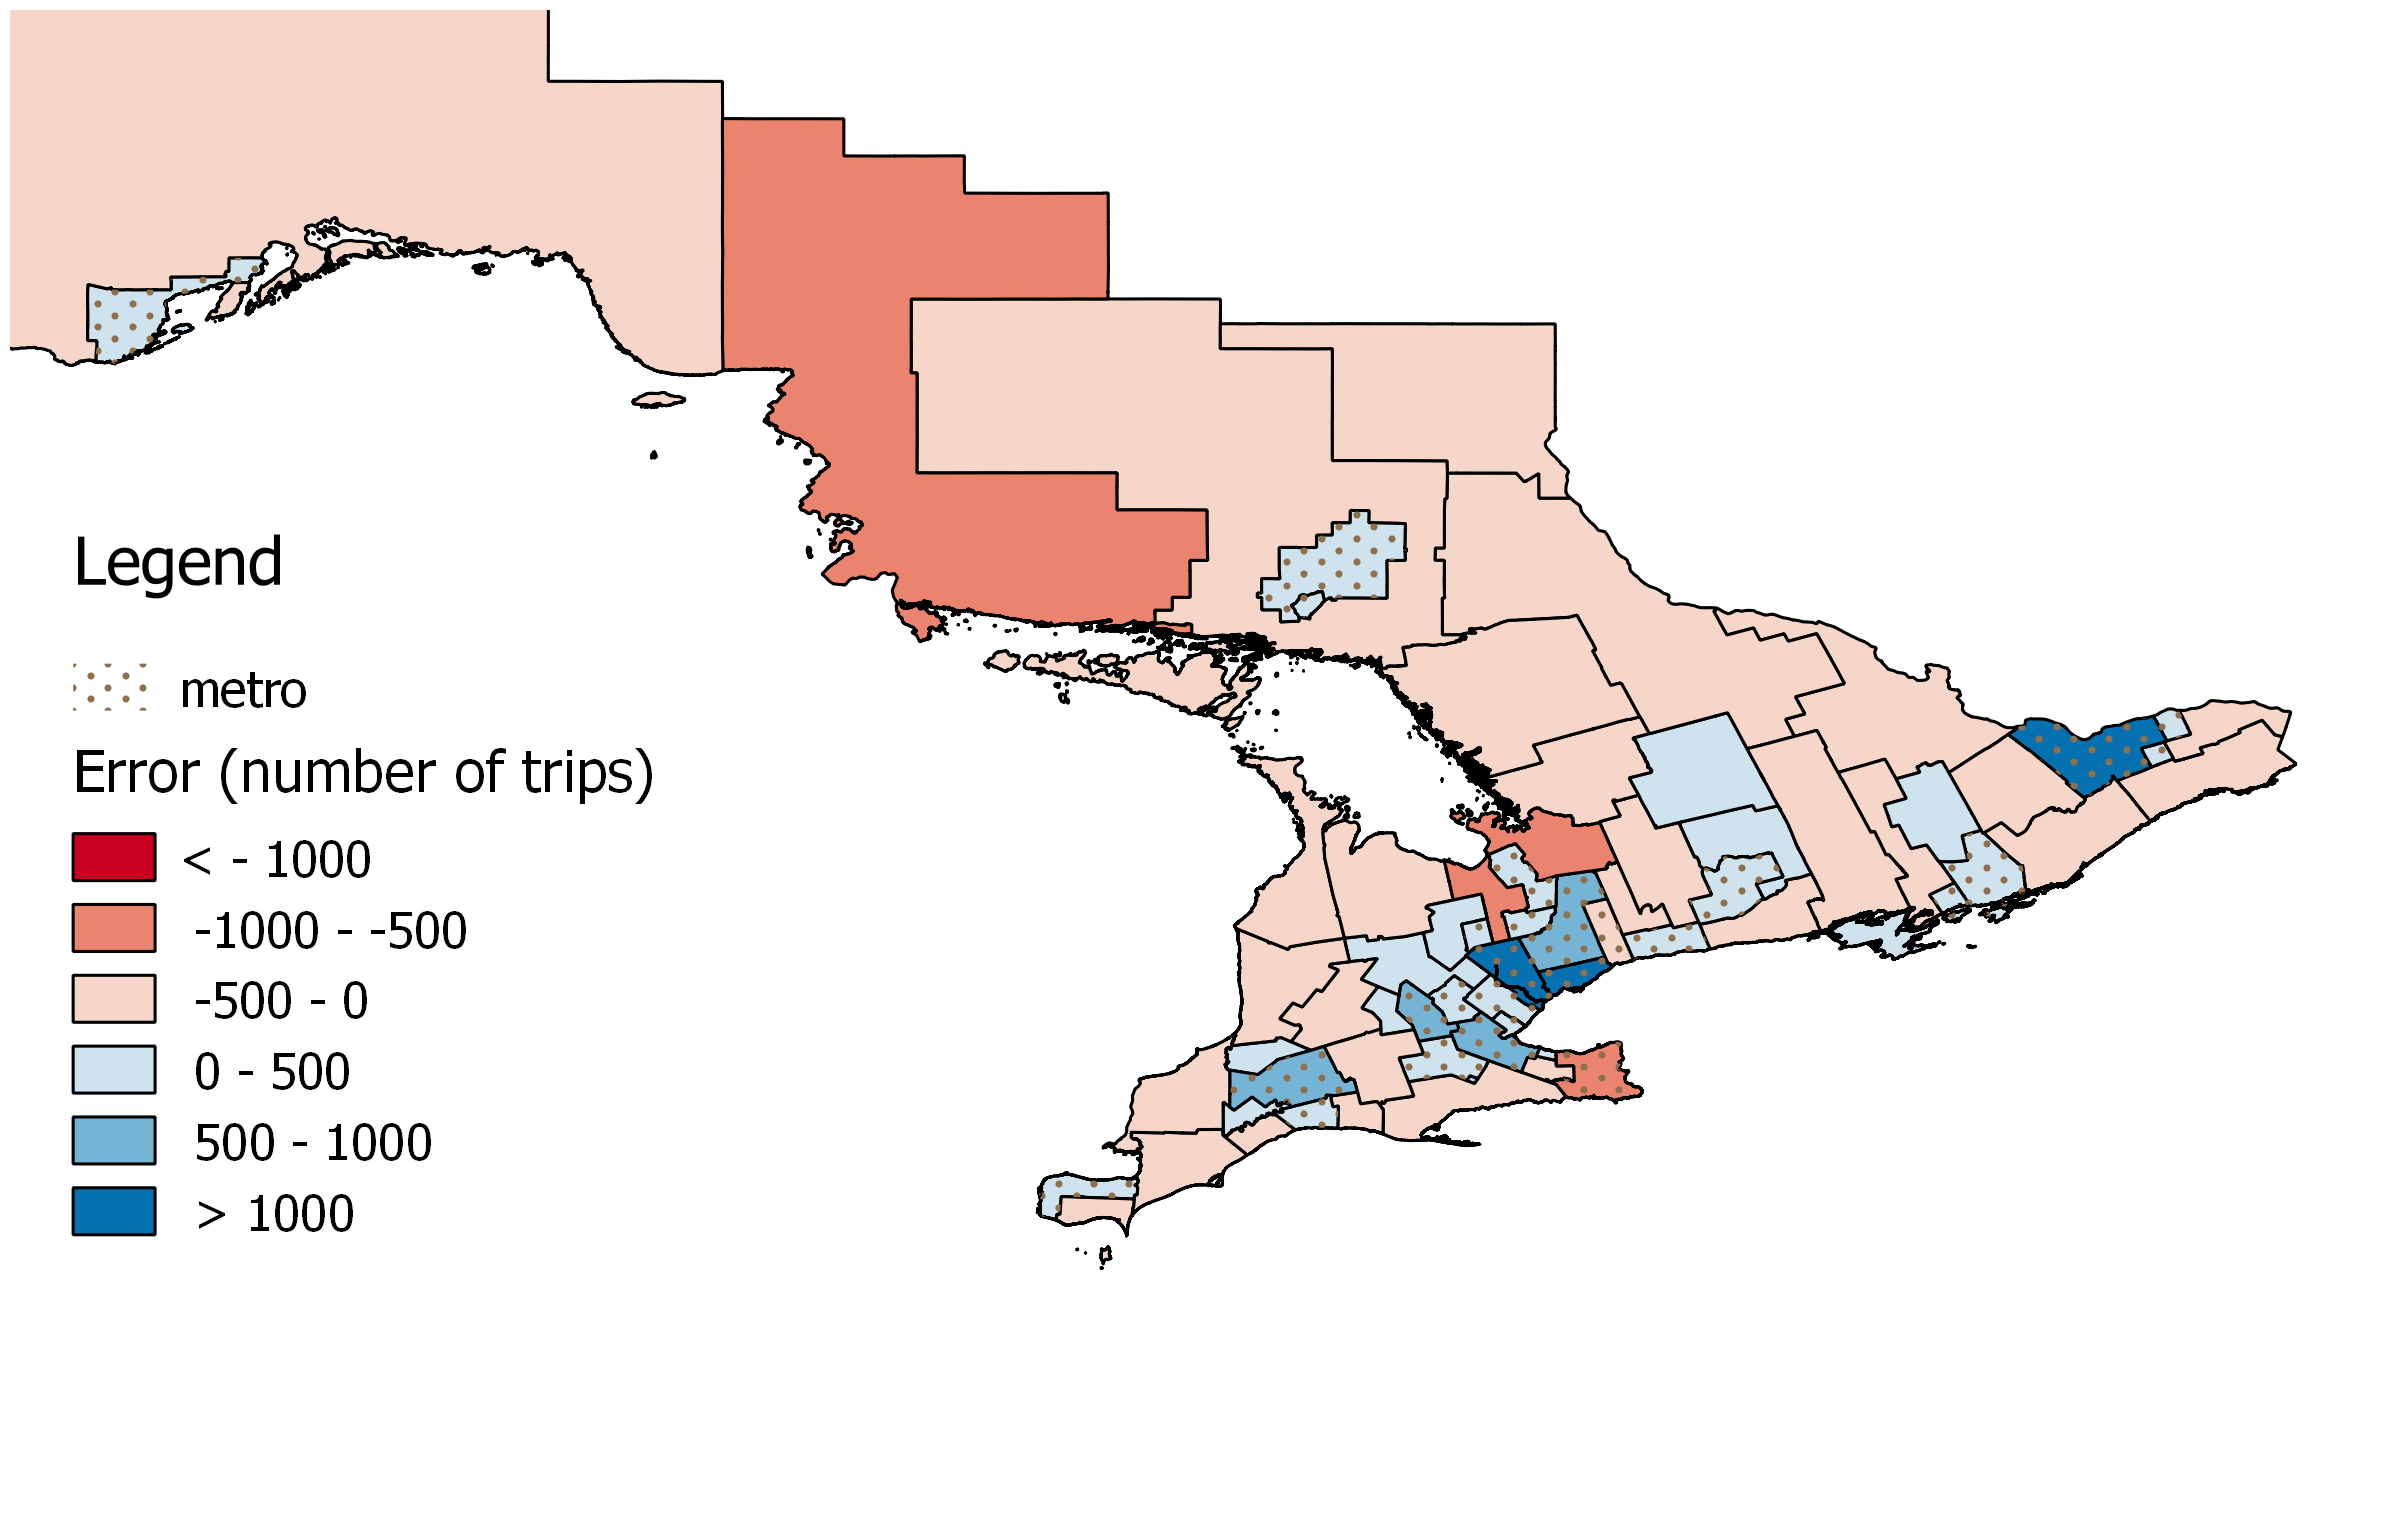
\includegraphics[width=\textwidth]{intrazonal_errors}
\caption{Intrazonal errors produced by the \textit{m2} model}
\label{fig:m2-intrazonal}
\end{figure}

\begin{figure}[H]
\centering
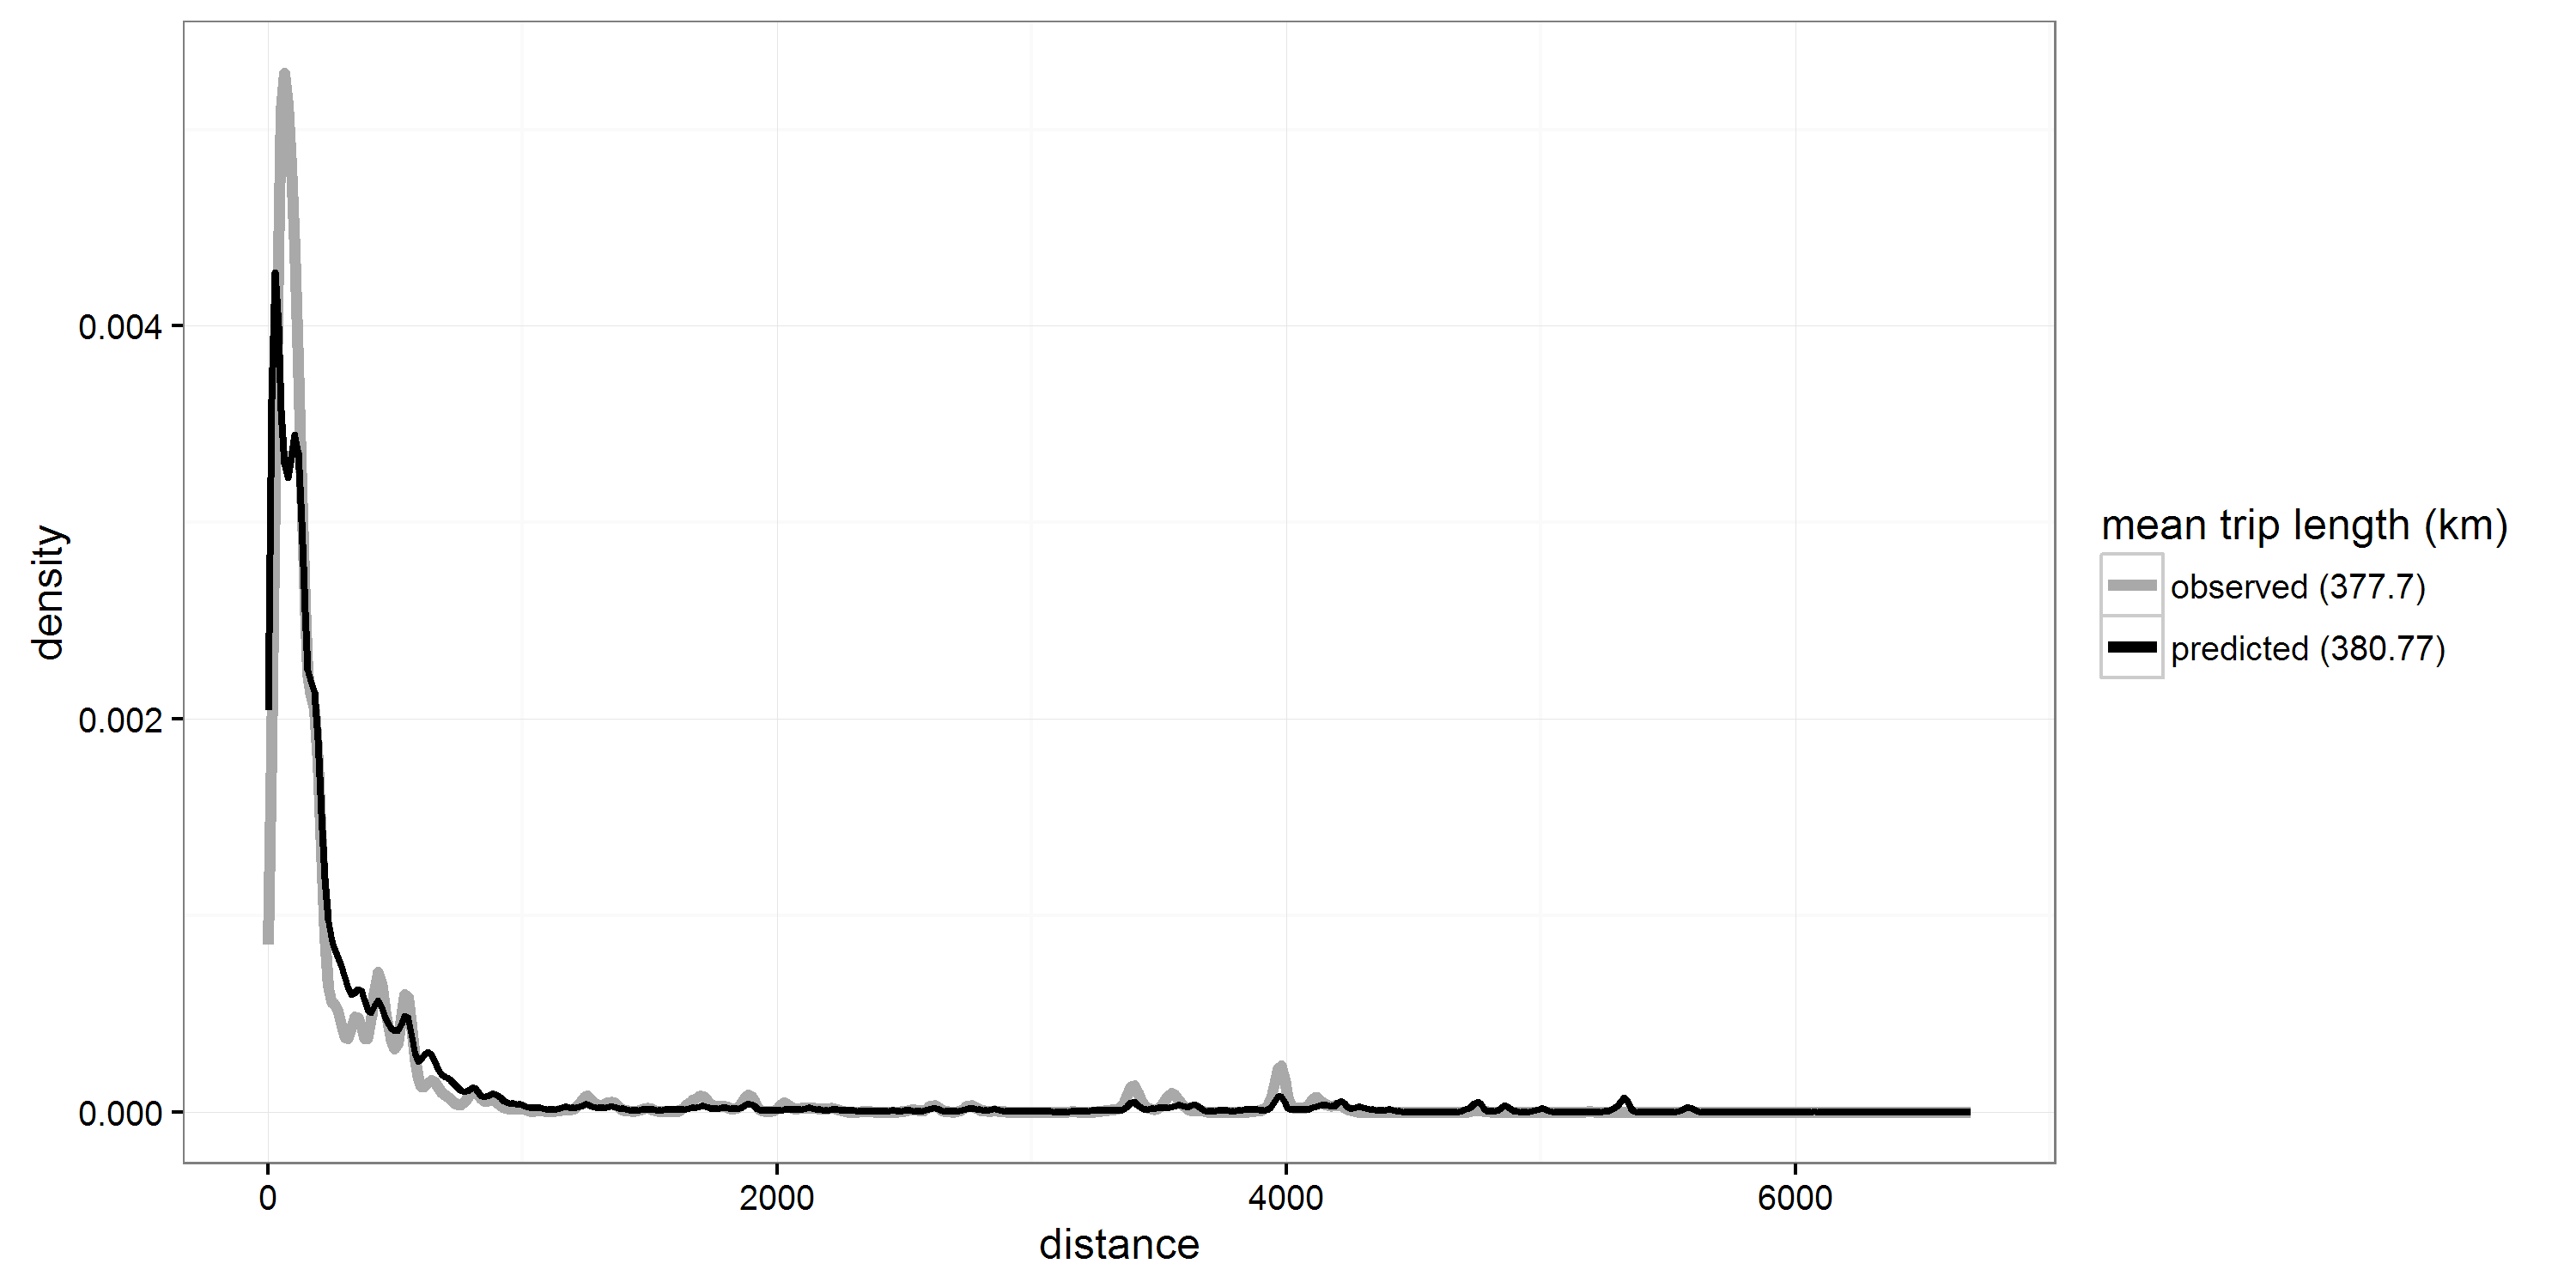
\includegraphics[width=0.8\textwidth]{calibration/m6_calibrated_business}
\caption{Trip length distribution of calibrated model for business travel}
\label{fig:calibration-business}
\end{figure}


\begin{figure}[H]
\centering
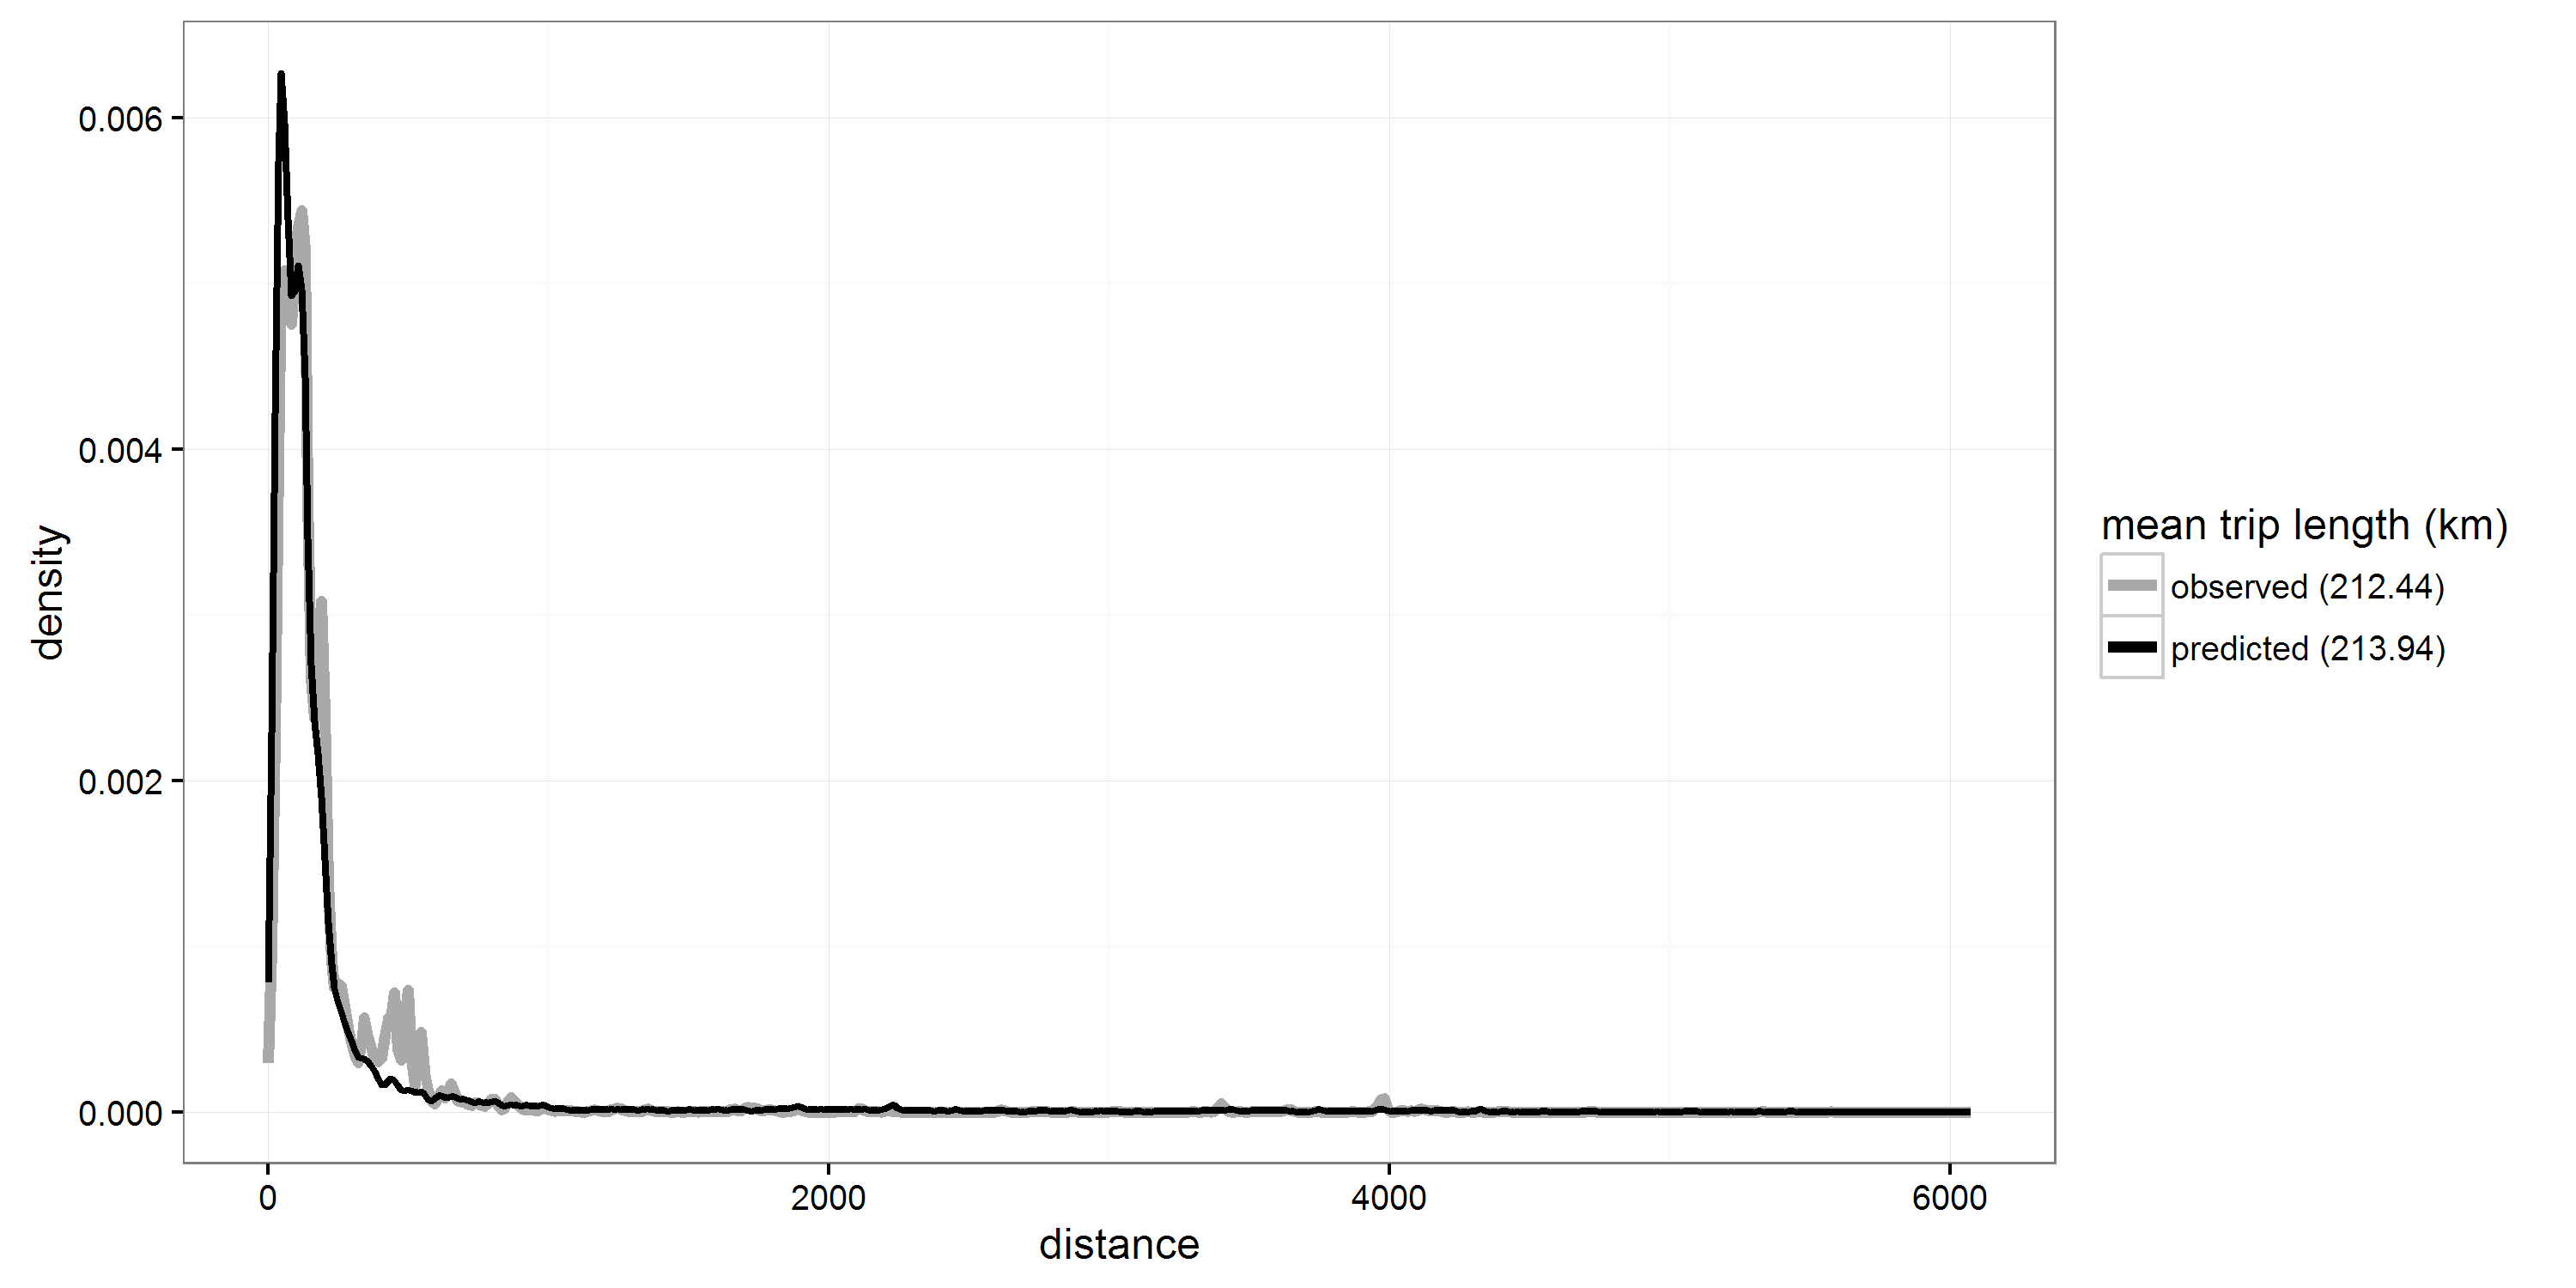
\includegraphics[width=0.8\textwidth]{calibration/m6_calibrated_leisure}
\caption{Trip length distribution of calibrated model for leisure travel}
\label{fig:calibration-leisure}
\end{figure}


\begin{figure}[H]
\centering
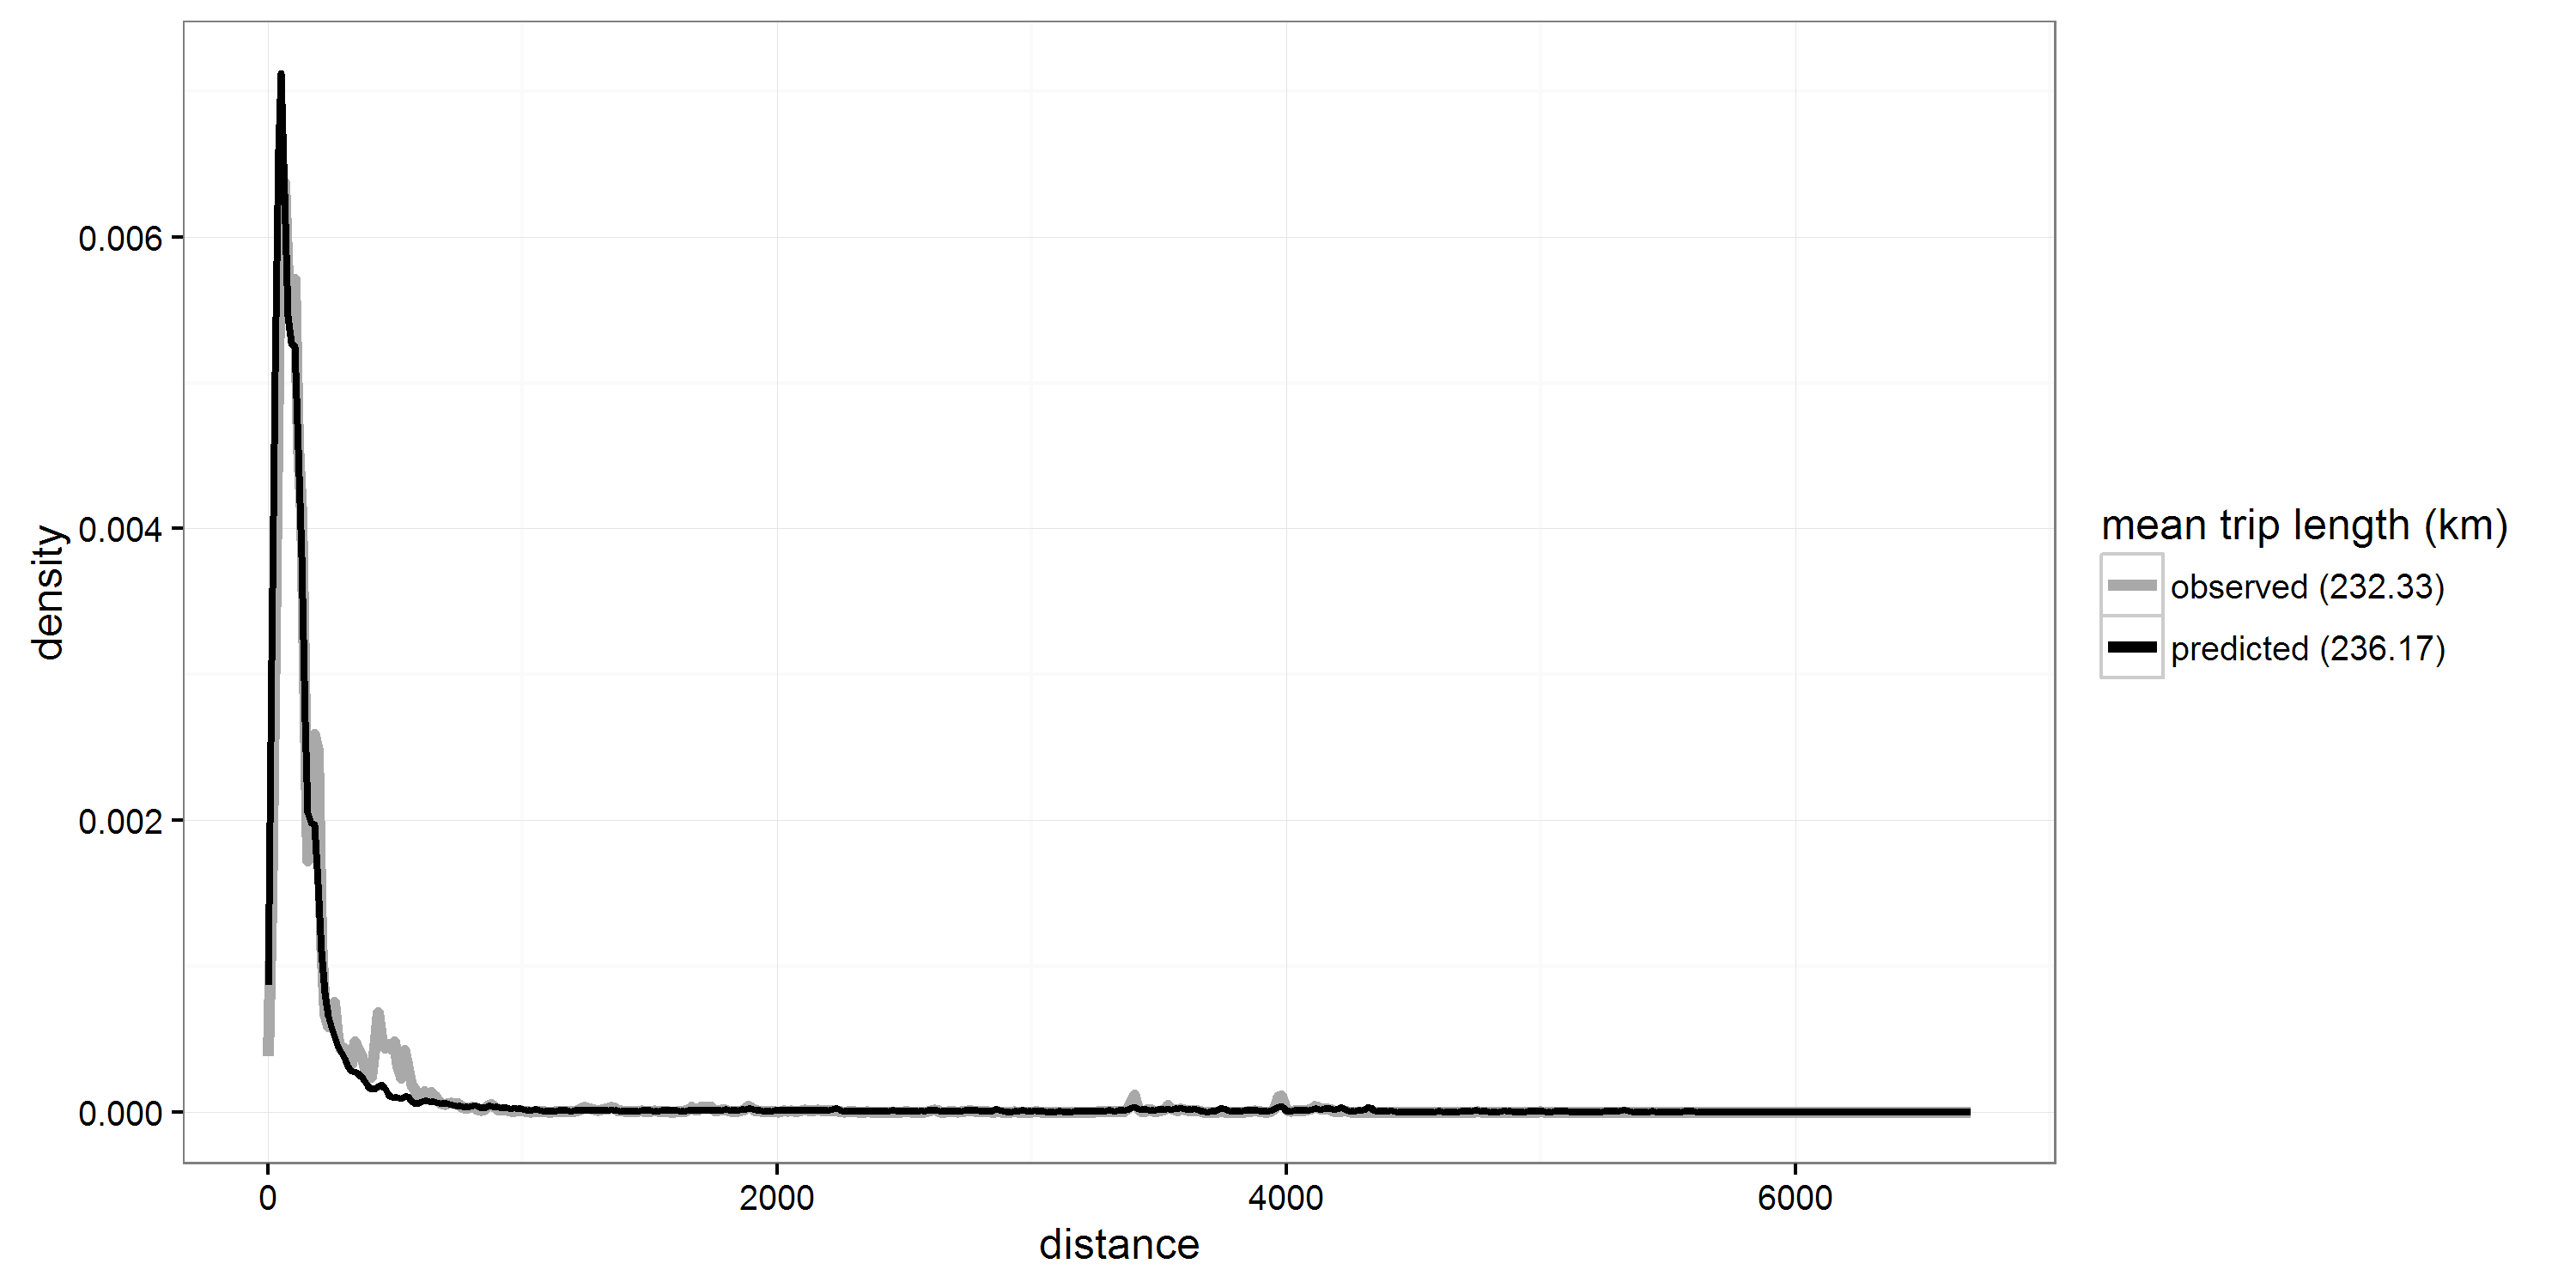
\includegraphics[width=0.8\textwidth]{calibration/m6_calibrated_visit}
\caption{Trip length distribution of calibrated model for visit travel}
\label{fig:calibration-visit}
\end{figure}

\begin{table}[ht]
\caption{Scenario Analysis results, incoming trips to zone 24: Dufferin (Toronto)}
\label{table:scenario-results}
\centering
% Table generated by Excel2LaTeX from sheet 'Sheet2'
\begin{tabular}{lrrrr}
Scenario & business & leisure & visit & total\\
\midrule
pre ski resort & 573   & 2345  & 5183  & 8101 \\
\midrule
civic & 577   & 2341  & 5241  & 8159 \\
hotels & 775   & 3895  & 6396  & 11066 \\
outdoors (summer only) & 776   & 4802  & 6351  & 11929 \\
skiing (winter only) & 773   & 5532  & 6357  & 12662 \\
   \bottomrule
\end{tabular}%

\end{table}



